\chapter{Thiết lập thực nghiệm và Đánh giá\label{chapter:eval}}

\section{Cấu hình testbed\label{sec:testbed}}
Hai môi trường thực thi phải được phân biệt, vì luận văn cố ý báo cáo
kết quả với hai mức sức nặng bằng chứng khác nhau, và phân biệt hoàn toàn phụ thuộc nơi
chúng được tạo ra.

\paragraph{Môi trường đã dùng.}
Mọi kết quả hiệu năng báo cáo trong chương này được đo trên một máy chủ dual-socket
chuyên dụng: hai bộ xử lý Xeon E5-2680~v4, $16$ vCPU trên một núm NUMA trình bày một luồng
mỗi lõi, chạy Rocky Linux~8.10 với \texttt{g++~15.1.1} và \texttt{rustc~1.97}. Benchmark
được ghim tới lõi $2$--$15$, để mỗi worker và mỗi producer sở hữu một lõi và
không tranh với hệ điều hành. Bảng~\ref{tab:testbed} liệt kê máy chủ so với
protocol mô tả dưới đây. Mỗi lần chạy ghi bản ghi môi trường riêng (mô hình CPU và topology, kernel, phiên bản compiler và toolchain, và
cài đặt tần số, turbo, và multithreading) cùng dữ liệu đo, nên điều kiện
của một phép đo đi cùng nó.

Một tính chất của máy này phải nói thẳng, vì nó giới hạn mọi luận điểm đuôi dưới đây: đó
là máy ảo. Bản ghi môi trường xác định guest KVM, và ba hệ quả
theo sau. Thứ nhất, governor tần số CPU và trạng thái turbo do host điều khiển. Chúng không
chỉ chưa đặt mà không quan sát được từ trong guest, nên ổn định tần số được giả định chứ không
bị ép. Thứ hai, bản ghi cho thấy CPU steal khác không, khoảng mười millisecond thời gian vCPU
mỗi giây. Nhỏ theo tổng, nhưng cùng bậc độ trễ đuôi được đo, và không gì trong guest có thể loại bỏ. Thứ ba, topology không như vẻ ngoài.
Guest được hiện hai
socket tám lõi single-threaded, không phải hình dạng E5-2680~v4, phần mười bốn lõi
có simultaneous multithreading. Topology do đó là tổng hợp. Mười sáu vCPU có nằm trên lõi vật lý riêng hay chia thread sibling là quyết định host, và
không đọc được từ trong guest. Sibling sẽ tranh tài nguyên thực thi của một lõi.
Lõi cũng không bị gỡ khỏi scheduler bằng
\texttt{isolcpus}, nên luồng benchmark vẫn có thể mất lõi cho việc khác.

Đây là công cụ tốt hơn nhiều so với laptop phát triển dùng chung mà lượt trước của
chiến dịch dùng. Lõi đồng nhất và server-class, không có gì quan trọng khác
chạy trên máy, và spread run-to-run ở p99 giảm hơn một bậc
magnitude giữa hai lần. Vẫn không phải máy bare-metal mà protocol dưới đây chỉ định.

\paragraph{Protocol mà chiến dịch hiệu năng vẫn thiếu.}
Số đuôi cấp testbed cần máy bare-metal chuyên dụng. Protocol cho một máy như vậy
được chỉ định, viết script, và công bố, nên có thể chạy không cần thiết kế thêm
(\texttt{bench/TESTBED.md}), và yêu cầu nằm ở cột phải của
Bảng~\ref{tab:testbed}. Việc chạy sẽ bổ sung hẹp hơn trước. Ba trong bốn
thứ nó sẽ mua đã có không cần nó: knee bão hòa, hình dạng
vách quá tải
(Mục~\ref{sec:overload}), và tái lập so sánh tài nguyên qua đối chứng bộ cấp phát
(Mục~\ref{sec:resources}). Còn lại là đuôi xa \emph{dưới} bão hòa.
Ở đó khoảng tin cậy trên p99 của một variant đơn vẫn nhiều lần spread giữa
cả bốn variant, và nguyên nhân có thể là steal và preemption scheduler, không
phải gì hai ngôn ngữ làm. Kết quả đó do đó được báo là chưa giải quyết chứ không
là null, và máy phải sửa, không phải phân tích.

\paragraph{Kỷ luật đo lường chung cho cả hai.}
Dù host nào, mỗi điểm sweep được lặp \NRepeats{} lần và báo là
median với khoảng tin cậy bootstrap $95\%$, không bao giờ một lần chạy. Bốn
variant ngôn ngữ$\times$bộ cấp phát được xen kẽ trong mỗi lần lặp, nên trôi nhiệt hoặc
nền không cân bằng chúng như nhau thay vì thiên một bên. Xen kẽ đó là điều làm
host tranh chấp dùng được cho kết luận \emph{so sánh} dù phá hỏng
số tuyệt đối, vì nhiễu khi đó được chia sẻ chứ không gán. Throughput được đếm
chỉ trong giai đoạn đo, bỏ warm-up khỏi cả mẫu số và
tử số, nên throughput đạt được so trực tiếp với tải đề nghị.

Phân chia Bảng~\ref{tab:testbed} vẽ không phải giữa kết quả quan trọng và không quan trọng. Nó
là giữa kết quả là tính chất của compiler và nguồn, mà host này thiết lập
chắc như mọi host, và kết quả là tính chất của máy, mà nó không thể
thiết lập.

\section{Workload và phép đo đánh giá\label{sec:workload}}
Workload viễn thông tổng hợp nhưng có căn đặc tả được tạo bởi driver quyết định mà
cấu trúc cả hai triển khai chia sẻ, nên hai bản được kích hoạt qua cùng
đường mã. Hai workload được cung cấp. Workload \emph{signal} preload quần UE
đã kết nối rồi đập đường nóng \texttt{handle\_signalling}, cô lập
độ trễ mỗi thông điệp ổn định. Workload \emph{mixed} là generator vòng đời RAN ghim.
Nó đi mỗi UE qua chuỗi thủ tục thực tế, tạo ngữ cảnh, thiết lập kết nối,
signalling, thiết lập bearer, reconfiguration/handover (begin/complete/abort), và release, dùng
thứ tự vẽ SplitMix64 cố định và mô hình trạng thái mong đợi theo slot để mọi thao tác phát ra
hợp lệ. Thứ tự vẽ cố định nghĩa số đếm theo loại thao tác giống hệt trong C++ và
Rust cho quần UE hoạt động và seed cho trước, đóng vai tín hiệu parity mô tả ở
Mục~\ref{sec:parity}. Tham số điều khiển là tốc độ sự kiện mục tiêu và số
UE hoạt động, sweep từ tải danh nghĩa qua bão hòa và quá tải. Lịch gửi cố định
và histogram được hiệu chỉnh, nên stall không gây bias coordinated-omission~\cite{schroeder2006openclosed,tene_hdrhistogram}. Ba chiến dịch đo được chạy: sweep tải cho
hiệu năng, nghiên cứu tiêm lỗi, và prototype migration FFI.
Hình~\ref{fig:workload} cho thấy hai workload và chuỗi thủ tục workload mixed
đi qua.

\begin{figure}[ht]
\centering
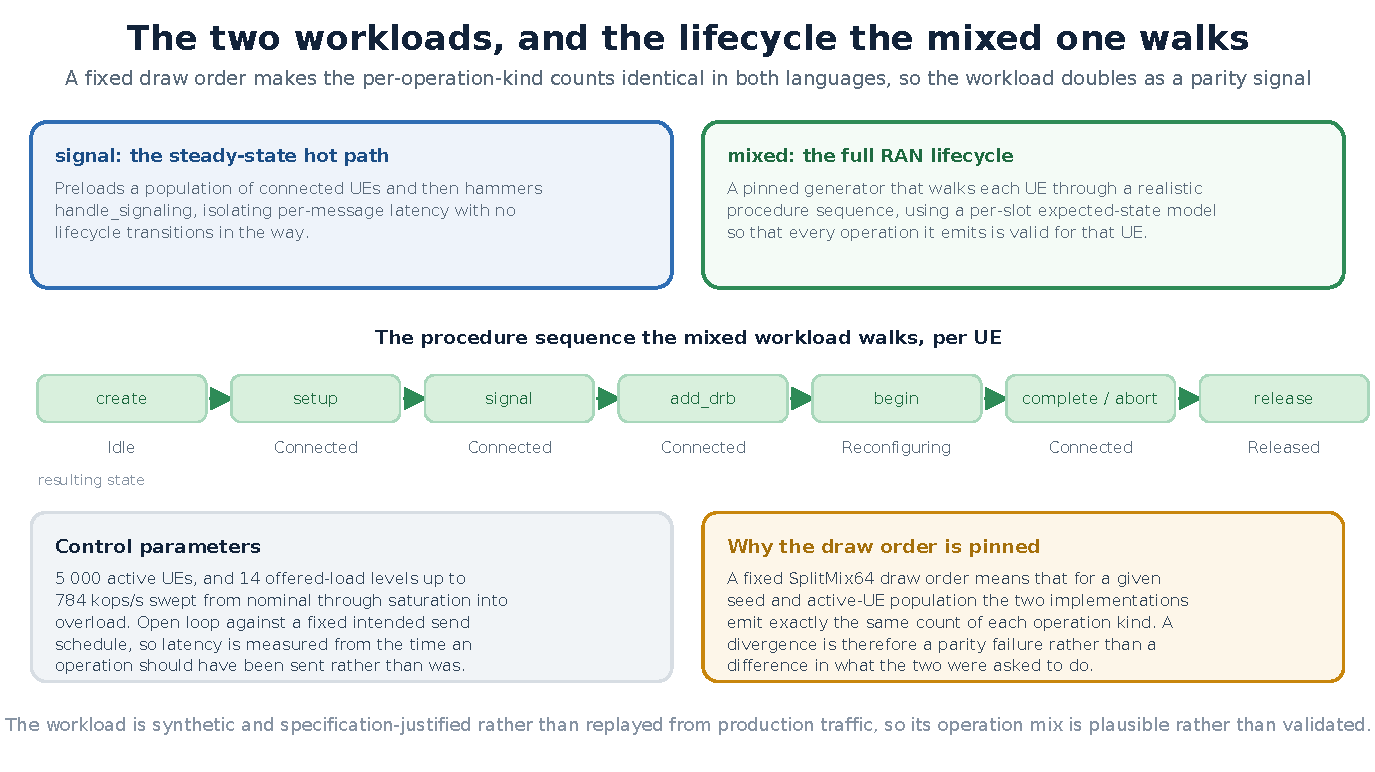
\includegraphics[width=0.78\linewidth]{diagrams/pdf/27_workload_timeline.pdf}
\caption[Hai workload và vòng đời workload mixed đi qua]{Hai workload. Workload \emph{signal} cô lập đường nóng ổn định.
Workload \emph{mixed} đi mỗi UE qua toàn chuỗi thủ tục RAN, với
mô hình trạng thái mong đợi theo slot đảm bảo mọi thao tác phát ra hợp pháp với trạng thái
ngữ cảnh thực sự ở. Vì thứ tự vẽ SplitMix64 được ghim, seed và
quần UE hoạt động cho trước tạo số đếm theo loại thao tác giống hệt ở cả hai ngôn ngữ, nên
phân kỳ là thất bại parity chứ không phải khác biệt trong việc hai triển khai được
yêu cầu làm.\label{fig:workload}}
\end{figure}

\paragraph{``Có căn đặc tả'' khẳng định gì, và không khẳng định gì.}
Thuật ngữ được dùng chính xác, vì phân biệt giới hạn workload hỗ trợ gì. \emph{Chuỗi}
thao tác được biện minh. Đó là vòng đời kết nối RRC mà đặc tả 3GPP
định nghĩa cho UE, từ thiết lập qua signalling trong phiên và thiết lập bearer
đến reconfiguration và release~\cite{3gpp38401,3gpp38331}. Mô hình trạng thái mong đợi theo slot sau đó
đảm bảo mọi thao tác driver phát ra hợp pháp với trạng thái ngữ cảnh thực sự ở,
nên workload không đẩy dịch vụ xuống đường đặc tả cấm. \emph{Tỷ lệ}
không được biện minh cùng cách. Tần suất cell thực handover so với
thiết lập bearer phụ thuộc triển khai, mobility, và thời điểm trong ngày, và không
có số công khai cố định. Mix dùng ở đây do đó hợp lý chứ không được xác thực.
Mục~\ref{sec:threats} báo đó là mối đe dọa tính ngoại sinh, và replay trace đứng đầu
danh sách công việc tương lai vì lý do này.

Với câu hỏi \emph{so sánh}, phân biệt ít tốn hơn so với câu tuyệt đối,
và nói vì sao là phần lập luận dữ liệu phù hợp nhiệm vụ. Cả hai triển khai thực thi
cùng chuỗi cùng thứ tự cho seed và quần UE hoạt động cho trước, và
số đếm theo loại thao tác xác minh. Mix không đại diện do đó dịch chuyển cả hai ngôn ngữ
bằng nhau và không thể tạo khác biệt giữa chúng. Mix thao tác chưa xác thực giới hạn số
đi xa bao nhiêu. Nó không làm suy yếu công bằng của so sánh chúng được dùng tạo.

Bảng~\ref{tab:params} gom cấu hình dịch vụ, workload và chiến dịch ở
một chỗ. Các giá trị đó nếu không gom sẽ rải qua đặc tả,
Chương~\ref{chapter:design}, và chương này. Tiện khi đọc từng phần, và
khó cho ai muốn tái lập chiến dịch hoặc đánh giá tham số có chọn để
phù hợp kết quả. Mỗi mục trong khối chiến dịch hoặc cố định bởi đặc tả hoặc
tạo từ log đo, nên không phần nào lệch khỏi dữ liệu báo cáo
dưới đây. Hai giá trị suy ra được dùng xuyên suốt phần sau. Điểm vận hành đại diện
không chọn bằng mắt. Nó là tải sweep bận nhất mà cả bốn variant build vẫn giữ
p99 dưới $5$~ms, đặt nó ở $\ReprLoad$~kops/s, so với bão hòa đo
$\SatKnee$~kops/s.

\section{Dữ liệu đánh giá}
Ba chiến dịch tạo ba tập dữ liệu, và chúng khác loại chứ không chỉ nội dung. Phần
sau mô tả mỗi tập khi được ghi. Người đọc đánh giá phân tích có đúng cần
biết gì được ghi và ở mức chi tiết nào, không chỉ gì được báo. Mọi đại lượng đo
chương này trích dẫn đến trang là macro được tạo.
\texttt{bench/refresh\_thesis.sh} tái tạo tất cả, cùng mọi hình và thân bảng,
từ log thô, nên rerun di chuyển văn bản và không thể để số tiêu đề
bị bỏ lại. Proxy chất lượng
phần mềm không thu ở đây mà báo nơi đọc rõ nhất: cạnh log điểm bắt buộc nó giải thích (Bảng~\ref{tab:complexity}), và cạnh seam FFI, nơi duy nhất
một trong hai triển khai chứa \texttt{unsafe} (Bảng~\ref{tab:ffi}).

\paragraph{Sweep hiệu năng.}
Mỗi trong $\NRuns$ lần chạy của thiết kế factorial Bảng~\ref{tab:params} đóng góp một
bản ghi, viết dạng JSON newline-delimited. Chiến dịch do đó là log append-only chứ không phải
bảng tóm tắt. Không gì được gộp khi ghi, và mọi statistic chương này được
tính lại từ bản ghi thô. Bản ghi mang cấu hình lần chạy (ngôn ngữ, bộ cấp phát,
workload, số shard và producer, tốc độ mục tiêu), kết quả (thao tác hoàn tất, lỗi,
thời lượng wall-clock, throughput đạt), phân phối độ trễ đọc từ histogram HDR
(mean, p50, p90, p99, p99.9, maximum, nanosecond), counter tài nguyên qua
\texttt{getrusage} (peak RSS, giây CPU user và system, mức
sử dụng CPU), và số đếm theo loại thao tác. Giữ số đếm loại trong mọi bản ghi là
điều làm phân kỳ giữa hai ngôn ngữ hiện là thất bại parity
(Mục~\ref{sec:parity}) thay vì bị nhầm là khác biệt hiệu năng.

\paragraph{Phân rã thành phần và nguyên thủy tranh chấp.}
Cấp đo thứ hai Mục~\ref{sec:methodperf} cho tập dữ liệu nhỏ hơn nhiều, hình dạng
khác. Với mỗi trong \BudgetRepeats{} lần lặp xen kẽ nó ghi chi phí batch-mean
ở cả hai ngôn ngữ, một lần gọi thao tác trực tiếp và một lần cùng thao tác qua
dịch vụ có luồng. Tập thứ ba, cùng hình ghép qua \ContentionRepeats{} lần lặp, ghi
throughput bền vững qua hàng đợi có giới hạn và nguyên thủy hoàn tất riêng
(Mục~\ref{sec:contention}). So sánh FFI Mục~\ref{sec:migrationresults} có
cùng cấu trúc qua \FfiOpRepeats{} lần lặp. Cả ba được ghép theo cấu trúc, điều test ghép chính xác
Mục~\ref{sec:stats} yêu cầu.

\paragraph{Catalogue tiêm lỗi.}
Tập dữ liệu này là phân loại chứ không số. Mỗi trong $\FaultClasses$ trường hợp lỗi cho bốn
log
công cụ: output AddressSanitizer, ThreadSanitizer và UndefinedBehaviorSanitizer cho chương trình C++,
và output \texttt{rustc} cho bản Rust an toàn tương ứng. Mỗi trường hợp cũng cho một
dòng taxonomy máy đọc được, ghi ba kết quả sanitiser, giai đoạn phát hiện,
kết quả compiler với mã chẩn đoán kích hoạt, và kỳ vọng đăng ký trước
nghiên cứu. Hai trường hợp boundary gốc cho bảng thứ hai từ model checker, và
\texttt{unsafe} một bảng thứ ba từ interpreter. Mang
kỳ vọng trong dữ liệu thay vì trong văn bản là điều cho runner báo mismatch
theo cả hai chiều. Bảng và hình Mục~\ref{sec:safetyresults} được tạo từ
file đó, không chép từ nó.

\paragraph{Điều đi cùng dữ liệu.}
Mỗi chiến dịch viết bản ghi môi trường cạnh kết quả. Nó ghi host và kernel,
distribution, phiên bản compiler và toolchain, mô hình CPU và topology, và governor tần số,
turbo, và cài đặt simultaneous-multithreading, \emph{kể cả} trường host cho trước
không expose. Chi tiết cuối quan trọng hơn nghe. Bản ghi xác định host
là guest KVM, và governor và turbo được lưu unavailable thay vì bỏ
đi. Hạn chế Mục~\ref{sec:testbed} tài liệu do đó là tính chất của tập dữ liệu
chứ không chỉ văn bản mô tả, và người đọc có thể kiểm tra không cần tin.

Tập dữ liệu hiệu năng đầy đủ và tự nhất quán cho phân tích và được dùng dưới đây để
trả lời RQ1 và RQ3 tạm thời. Chạy lại cùng script trên chiến dịch ghi trên
máy bare-metal thay các số bằng số cấp testbed không thay đổi
phân tích.

\section{Kết quả đánh giá}
Kết quả an toàn và migration không phụ thuộc máy đo. Kết quả hiệu năng và
tài nguyên phụ thuộc, và Mục~\ref{sec:testbed} nêu máy đó mang và không mang gì.
Mọi hình và bảng dưới đây được đo trên nó trừ khi nói khác.

Kết quả đã giải quyết và chưa giải quyết được báo cạnh nhau. Nói ngay đầu cái nào là gì
ngăn kết quả null bị đọc như không có. Sáu phát hiện đã giải quyết: taxonomy
lớp lỗi và ranh giới (Mục~\ref{sec:safetyresults}), chi phí seam FFI
(Mục~\ref{sec:migrationresults}), khác biệt bộ nhớ giữa hai build
(Mục~\ref{sec:resources}), chi phí thao tác thuần (Mục~\ref{sec:budget}), tương đương bốn variant ở median dưới bão hòa, và phân kỳ qua nó
(Mục~\ref{sec:overload}). Cái cuối là hiệu ứng ngôn ngữ lớn nhất và tái lập nhất
trong nghiên cứu.

Đuôi xa \emph{dưới} bão hòa là kết quả chưa giải quyết duy nhất, và host là lý do.
Spread run-to-run ở p99 vượt mọi khác biệt giữa variant, và không số lần lặp
trên máy ảo với CPU steal khác không đóng khoảng đó
(Mục~\ref{sec:perfresults}). Chỉ protocol bare-metal Mục~\ref{sec:testbed} sẽ
trả lời. Phân kỳ quá tải được giải quyết như phép đo, dù chưa đầy như cơ chế.
Mục~\ref{sec:contention} kiểm tra hàng đợi có giới hạn và nguyên thủy hoàn tất riêng
có giải thích không. Chúng không tái tạo thứ tự full-service ở mức ý nghĩa, để lại
việc ở đâu đó trên toàn đường handoff ngoài nguyên thủy cô lập.

\subsection{Hiệu năng (RQ1, RQ3)}\label{sec:perfresults}
Giả thuyết được thử là H1: hai ngôn ngữ tương đương hiệu năng dưới
bão hòa, mọi khác biệt chỉ ở đuôi xa. Mục này báo nơi, nếu
có, mỗi bên thắng và bao nhiêu, qua sweep tới và qua bão hòa.

Mọi thứ trong mục được tạo từ log thô bởi \texttt{bench/plot\_figures.py}: hình,
bảng, và số trích trong văn bản. Mục do đó có thể tái tạo
nguyên văn nếu chiến dịch rerun trên testbed bare-metal. Số tuyệt đối thuộc
host Mục~\ref{sec:testbed}. Mỗi điểm gộp \NRepeats{} lần lặp xen kẽ.
Giá trị bảng và dải shaded là median với khoảng tin cậy bootstrap $95\%$
nonparametric.

Bảng~\ref{tab:latency} tóm tắt phân phối độ trễ mỗi thao tác ở tải đề nghị
bền vững $\ReprLoad$~kops/s. Điểm vận hành không chọn bằng mắt: nó là
tải sweep cao nhất mà mọi một trong bốn variant build vẫn giữ p99 dưới
$5$~ms, tức điểm bận nhất mà cả bốn cùng khỏe, làm
nó nơi công bằng nhất để so sánh.

Bảng phải đọc ở hai mức tin cậy khác nhau, và tách chúng là
cách đọc trung thực của chiến dịch. Ở \emph{median} bốn variant nằm trong
$\PFiftyRange\,\mu$s của nhau, hay $\PFiftySpread\%$, và mọi cặp khoảng tin cậy
giao nhau. Bảng đơn lẻ do đó không phân tách gì.
Đó là câu về khoảng không ghép chứ không về ngôn ngữ. Test ghép
dưới đây giải quyết khác biệt nhỏ và nhất quán ở median, và khoảng giữa
hai cách đọc chính xác là lý do Mục~\ref{sec:stats} test so sánh thay vì
nhìn khoảng.

\emph{Trên} median tình huống khác loại. Điểm không phải ngôn ngữ khác mà host này không thể nói có khác không. Giá trị p99 khác
$\PNineNineRange\,\mu$s giữa variant, trong khi khoảng tin cậy $95\%$ rộng nhất trên
p99 của một variant đơn trải $\PNineNineMaxCI\,\mu$s, nhiều lần khác biệt
giữa variant. Khi uncertainty về một variant vượt khoảng giữa cả bốn, không
thứ tự nào đọc được. Báo một sẽ là báo scheduler. Cùng điều
mạnh hơn ở p99.9 và maximum.

Đây là dạng cụ thể của hạn chế Mục~\ref{sec:testbed} nêu, và chi phí được
giới hạn. Nó không chạm throughput và hành vi bão hòa, kết quả tài nguyên dưới đây,
hay gì trong chương RQ2 và RQ4. Nó nghĩa là một nửa RQ1 chỉ nhận
câu trả lời phủ định từ chiến dịch này, tức hai ngôn ngữ hành xử thế nào ở percentile cao
khi dịch vụ vẫn đáp ứng tải đề nghị. Đuôi đó chưa đo được. Nửa kia
không bị chạm, và Mục~\ref{sec:overload} giải quyết nó dứt khoát trên cùng host này.
Đóng khoảng cần protocol bare-metal, không thêm lần lặp ở đây, vì spread là
nhiễu hệ thống chứ không phải nhiễu lấy mẫu. Mục~\ref{sec:budget} cũng cho thấy
đại lượng ngôn ngữ có thể ảnh hưởng nằm hơn ba bậc magnitude dưới đại lượng
phép đo này giải quyết.

Một điều chỉnh về metric thuộc đây chứ không chỉ thảo luận tính hợp lệ. RQ1
nêu median, p99, p99.9, và maximum vì bốn đó là chiến dịch này cung cấp.
Harness cũng ghi jitter giữa thao tác và p99.99, và giữ histogram đuôi xa
sẽ phải gộp từ, nhưng chiến dịch báo ở đây trước instrumentation đó.
Khả năng dự đoán do đó được chứng minh ở p99 và p99.9 và không xa hơn. Đó là khoảng trong
bằng chứng chứ không trong thiết kế, và nó đóng với chiến dịch bare-metal mà luận điểm đuôi
đã chờ.

\begin{table}[H]
\centering
\small
\caption[Độ trễ mỗi thao tác ở tải đại diện]{Độ trễ mỗi thao tác ở tải đề nghị bền vững $\ReprLoad$~kops/s (workload
vòng đời RAN mixed, $7$ shard). Giá trị microsecond: median qua \NRepeats{}
lần lặp trên khoảng tin cậy bootstrap $95\%$ nonparametric. Khoảng in đầy đủ thay vì nửa rộng đối xứng vì nó
rất bất đối xứng ở các percentile này, và nửa rộng đủ che bound trên sẽ đặt bound dưới
dưới không.\label{tab:latency}}
% Tabular preamble and header are generated alongside the table body, so the table
% gains a p99.99 column when a campaign records one instead of the preamble falling
% one column short of the body it is wrapping. \LatencyTabular expands to the whole
% \begin{tabular}{...}: array's preamble scanner does not expand macros, so passing
% only the column specification would fail with "Illegal pream-token".
\LatencyTabular
\hline\hline
\LatencyHead \\
\hline
C++ (system alloc) & \mci{217.2}{163.8}{237.2} & \mci{355.1}{289.3}{389.4} & \mci{674.3}{395.3}{1538.0} & \mci{2170}{910}{5594} \\
C++ (jemalloc) & \mci{225.8}{181.1}{261.2} & \mci{410.1}{305.7}{11280.4} & \mci{1188}{544}{14213} & \mci{3590}{1472}{16291} \\
Rust (system alloc) & \mci{214.3}{191.6}{238.8} & \mci{376.3}{330.2}{3629.1} & \mci{1068}{504}{6955} & \mci{2404}{1129}{9667} \\
Rust (jemalloc) & \mci{208.4}{193.7}{223.1} & \mci{388.9}{342.3}{478.0} & \mci{763.4}{479.5}{4272.1} & \mci{2804}{1114}{7606}
\\
\hline
\end{tabular}
\end{table}

\paragraph{Test so sánh thay vì nhìn mắt.}
Khoảng giao nhau là công cụ yếu theo cả hai chiều, nên so sánh cũng được test
trực tiếp, theo thủ tục cố định Mục~\ref{sec:stats} và báo trong
Bảng~\ref{tab:significance}. Điều cho phép ghép là tính chất của chiến dịch này chứ
không của statistic. Bốn variant được xen kẽ trong mỗi lần lặp, nên
lần chạy $i$ của mỗi được đo trong cùng block dưới cùng điều kiện môi trường. Mọi
nhiễu block mang là chung cho cặp, và hủy trong hiệu của chúng. Đó là
thứ hai kỷ luật xen kẽ mua, ngoài lập luận công bằng nó được chọn
vì.

\begin{table}[tp]
\centering
\small
\caption[Test ghép hoán vị chính xác C++ so với Rust]{Test ghép hoán vị chính xác C++ so với Rust ở $\ReprLoad$~kops/s, với
bộ cấp phát giữ cố định. Hiệu ứng là median của \NRepeats{} hiệu ghép
(Rust~$-$~C++), hiển thị trên khoảng tin cậy bootstrap $95\%$. Statistic test là
mean của chúng. $p$ chính xác qua mọi $2^{\NRepeats}$ gán dấu, và cột cuối
áp dụng hiệu chỉnh Holm trên cả họ \NTests{} test. Sàn có thể đạt
là $\MinAttainableP$ chưa hiệu chỉnh và $\CorrectedFloor$ sau hiệu chỉnh. Các dòng được khối
theo tập tiêu chí Mục~\ref{sec:stats}: ghép cứu statistic ở khối trên, nên khoảng nhất quán ở đó là bằng chứng, trong khi percentile cao dưới được tính từ đúng thao tác nhiễu rơi vào, nên khoảng loại trừ không được đọc là phát hiện. Throughput đạt không được test, vì lý do
cùng mục, và xuất hiện trong Bảng~\ref{tab:resource}. Đo trên host Xeon ảo
Mục~\ref{sec:testbed}.\label{tab:significance}}
\begin{tabular}{@{}l l r r r@{}}
\hline\hline
Metric & Allocator & Effect (Rust $-$ C++) & $p$ & Holm \\
\hline
\rlap{\emph{Robust to interference on single operations}} & & & & \\
p50 latency (\textmu s) & system & \mci{-1.3}{-1.3}{-1.2} & 0.0000019 & 0.000027 \\
p50 latency (\textmu s) & jemalloc & \mci{-1.2}{-1.3}{-1.2} & 0.0000019 & 0.000027 \\
Peak RSS (MiB) & system & \mci{+1.4}{+1.2}{+1.7} & 0.0000019 & 0.000027 \\
Peak RSS (MiB) & jemalloc & \mci{+2.5}{+2.4}{+2.6} & 0.0000019 & 0.000027 \\
CPU utilisation (\%) & system & \mci{-5.1}{-6.7}{-4.7} & 0.0000019 & 0.000027 \\
CPU utilisation (\%) & jemalloc & \mci{-4.6}{-5.9}{-3.9} & 0.0000019 & 0.000027\\
\hline
\rlap{\emph{Determined by it: high percentiles}} & & & & \\
p99 latency (\textmu s) & system & \mci{-1}{-2}{-1} & 0.0000057 & 0.000027 \\
p99 latency (\textmu s) & jemalloc & \mci{-1}{-1}{-1} & 0.0000038 & 0.000027 \\
p99.9 latency (\textmu s) & system & \mci{-4}{-5}{-2} & 0.00016 & 0.00016 \\
p99.9 latency (\textmu s) & jemalloc & \mci{-2}{-4}{-2} & 0.0000095 & 0.000027
\\
\hline
\end{tabular}
\end{table}

\begin{figure}[ht]
\centering
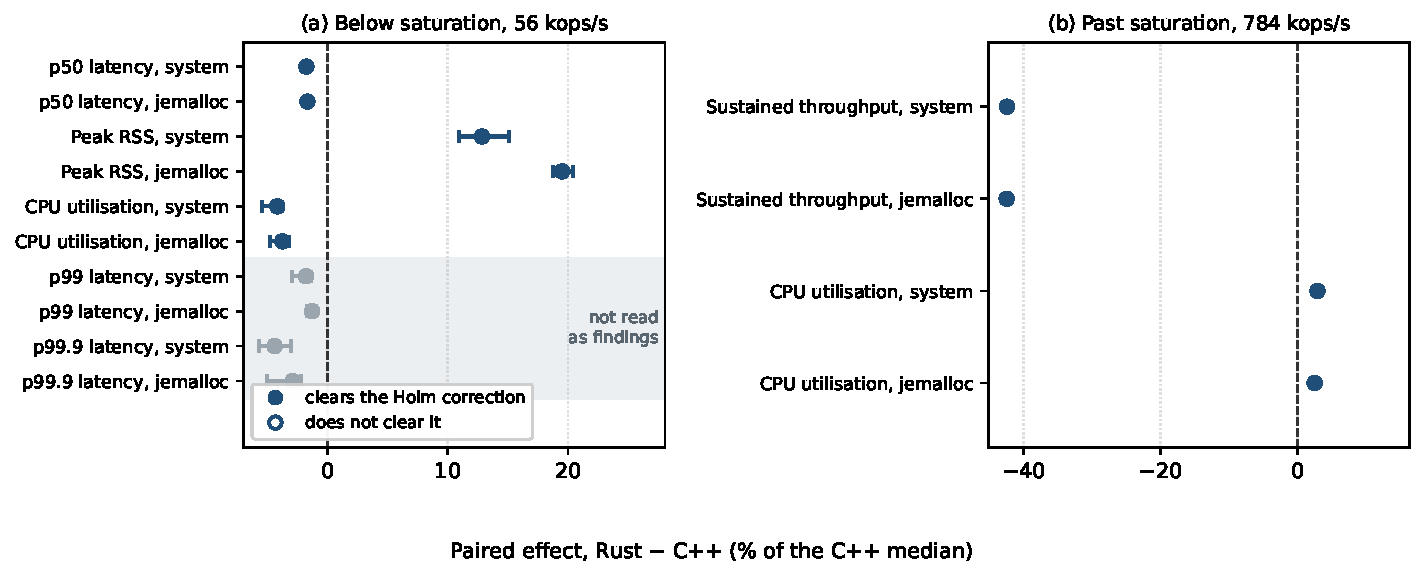
\includegraphics[width=0.78\linewidth]{figures/fig_effects.pdf}
\caption[Họ test được vẽ dưới dạng hiệu ứng ghép]{Mọi test trong Bảng~\ref{tab:significance} và~\ref{tab:overloadtest} dưới dạng hiệu ứng
ghép với khoảng bootstrap $95\%$, chuẩn hóa theo median C++ để microsecond,
mebibyte, điểm phần trăm và kops/s chia sẻ trục. Marker đầy là
\NSignificant{} trong \NTests{} test vượt hiệu chỉnh Holm. Hai bộ cấp phát của
metric được vẽ cạnh nhau, nên hiệu ứng đổi dấu giữa chúng sẽ hiện là cặp
qua đường không. Các dòng shaded là percentile cao, tính từ đúng thao tác nhiễu rơi vào, mà Mục~\ref{sec:stats} cố định trước là dòng có khoảng
không đọc là phát hiện. Metric giữ đơn vị riêng trong
bảng.\label{fig:effects}}
\end{figure}

Hình~\ref{fig:effects} vẽ cùng họ trên một trục, và ba điều trong đó
dễ thấy hơn trong bảng mười bốn dòng: hiệu ứng nào sống sót hiệu chỉnh,
hiệu ứng có giữ dấu khi bộ cấp phát đổi không, và khoảng đuôi
rộng hơn phần còn lại bao nhiêu.

Năm điều theo sau. Thứ nhất, \NSignificant{} trong \NTests{} test của họ sống sót hiệu chỉnh
Holm. Ở điểm vận hành này chúng là hai dòng median-latency, peak RSS
dưới bộ cấp phát hệ thống, và cả hai dòng CPU. Bốn còn lại sống sót là so sánh quá tải
Mục~\ref{sec:overload}. Peak RSS dưới jemalloc là dòng
khối trên duy nhất không vượt hiệu chỉnh, dù khoảng xa không, và
Mục~\ref{sec:resources} nói vì sao.

Thứ hai, quy tắc đọc cố định Mục~\ref{sec:stats} phải áp dụng trước khi diễn giải bất kỳ. \NExclZero{} khoảng ghép loại trừ không. Trong khối đuôi những loại trừ là: \TailExclZeroRows. Quy tắc được nêu trước, và không ở điểm này, chính xác
vì kết quả đó không được đảm bảo. Lượt trước bảy lần lặp cùng chiến dịch
đã tạo khoảng đuôi loại trừ không, và thêm lần lặp sau đó gỡ chúng. Đó là hành vi
quy tắc dự đoán.

Thứ ba, đối chứng bộ cấp phát cung cấp kiểm tra thứ hai, độc lập với thứ nhất. Mọi so sánh
chạy hai lần dưới điều kiện không nên đổi hiệu ứng ngôn ngữ, nên hiệu ứng thực sự
là ngôn ngữ nên giữ dấu dù liên kết bộ cấp phát nào. Ở đây
\CrossAllocConsistent{} tất cả giữ, và \NCrossAllocReversed{} đảo. Đối chứng xác nhận thay vì
phủ quyết không phải bằng chứng nó không cần. Trong chiến dịch trước, trước khi hai build \texttt{jemalloc} bị giữ một cấu hình, hiệu ứng CPU vượt hiệu chỉnh
dưới một bộ cấp phát và đảo dấu dưới bộ kia, và được báo chưa giải quyết theo
chính quy tắc này. Đối chứng kiếm chỗ bằng điều nó sẽ bắt, không phải điều nó
tình cờ bắt.

Thứ tư, \NEqvUnresolved{} dòng hiệu chỉnh không vượt không nói cùng một điều, và Bảng~\ref{tab:equivalence} là thứ tách chúng. Test không giải quyết khác biệt vẫn giới hạn nó: có margin chặt nhất trong đó hai variant có thể
gọi tương đương, và đó là tính chất dữ liệu chứ không phán quyết. Đọc vậy
khối trên và khối đuôi tách rõ. Ở median bound là
$\EqvBoundPFifty\,\mu$s, nên khác biệt test giải quyết cũng nhỏ theo tuyệt đối
và hai cách đọc đồng ý. Trong khối đuôi bound chạy tới $\EqvBoundTailMax\,\mu$s,
là khả năng host này không nhìn thấy được nêu dưới dạng số thay vì null. Phân biệt
quan trọng vì hai thứ thường được báo giống. Null với bound chặt là
kết quả. Null với bound rộng hơn mọi khác biệt triển khai quan tâm là
chiến dịch từ chối trả lời, và nói cái nào là điều tối thiểu bảng này làm cho nửa RQ1 host không thể giải quyết.

\begin{table}[H]
\centering
\small
\caption[Mỗi hiệu ứng có thể lớn bao nhiêu, cho so sánh test không giải quyết]{Mỗi hiệu ứng có thể lớn bao nhiêu. Với mọi so sánh ở $\ReprLoad$~kops/s,
hiệu ứng quan sát so với margin chặt nhất trong đó hai variant có thể gọi
tương đương, và phán quyết Bảng~\ref{tab:significance} đạt. Hai câu hỏi
cố ý giữ ở hai bảng: một hỏi khác biệt có ở đó không, bảng này hỏi nó
có thể lớn bao nhiêu nếu có, và một dòng có thể quan trọng ở một mà không ở bảng kia. Margin độ trễ là
microsecond, peak RSS mebibyte, sử dụng CPU điểm phần
trăm.\label{tab:equivalence}}
\begin{tabular}{@{}l l r r l@{}}
\hline\hline
Metric & Allocator & $|$Effect$|$ & Equivalent within & Verdict \\
\hline
p50 latency (\textmu s) & system & 1.2 & 1.3 & significant \\
p50 latency (\textmu s) & jemalloc & 1.5 & 1.6 & significant \\
p99 latency (\textmu s) & system & 2 & 2 & significant \\
p99 latency (\textmu s) & jemalloc & 1 & 1 & significant \\
p99.9 latency (\textmu s) & system & 4 & 4 & significant \\
p99.9 latency (\textmu s) & jemalloc & 3 & 3 & significant \\
Peak RSS (MiB) & system & 1.6 & 1.8 & significant \\
Peak RSS (MiB) & jemalloc & 2.5 & 2.5 & significant \\
CPU utilisation (\%) & system & 6.0 & 7.1 & significant \\
CPU utilisation (\%) & jemalloc & 6.2 & 7.3 & significant
\\
\hline
\end{tabular}
\end{table}

Thứ năm, median giờ là khác biệt đã giải quyết chứ không phải null: $\PFiftyDiffAbsMax\,\mu$s
theo hướng có lợi Rust, nhất quán dưới cả hai bộ cấp phát. Khoảng trên nó chạm
$\PFiftyDiffCIMax\,\mu$s so với median khoảng $80\,\mu$s, và cám dỗ là báo
đó là bound trên hiệu ứng ngôn ngữ. Cách đọc đó sai, và mục
sau giải thích vì sao.

\subsection{End-to-end số được ghép từ gì}\label{sec:budget}
Mọi độ trễ sweep báo là vòng quay end-to-end, và
Mục~\ref{sec:methodperf} nêu vì sao đó gói hai chi phí khác loại.
Một là thao tác, thực thi trong một luồng và do compiler tạo. Cái kia
là handoff gửi-và-hoàn tất qua luồng, tính cho hệ điều hành.
Chỉ cái đầu có thể khác giữa ngôn ngữ, và sweep không tách hai.

Điều quan trọng cho bound vừa trích, vì bound chỉ nói bằng đại lượng
nó là phần của. Cả hai chi phí do đó được đo trực tiếp, bằng phương pháp hai cấp
mô tả ở đó, ở cả hai ngôn ngữ và ở số shard và quần ngữ cảnh của sweep.
\texttt{ShardCore} gọi không có hàng đợi trên đường cho thao tác. \texttt{Service} cho
thao tác cộng handoff. Hiệu của chúng là handoff.
Bảng~\ref{tab:budget} cho kết quả, và nó định hình lại toàn so sánh hiệu năng.

\begin{table}[H]
\centering
\small
\caption[Chi phí end-to-end thực sự đi đâu]{Chi phí end-to-end thao tác thực sự đi đâu, đo ở $7$ shard và
$5\,000$ UE hoạt động với một caller không tranh chấp. Mỗi dòng là median qua
\BudgetRepeats{} lần lặp xen kẽ trên khoảng tin cậy bootstrap $95\%$, theo
đơn vị magnitude gọi: hai thành phần khác hơn hai bậc magnitude,
điểm của bảng. $p$ là test ghép hoán vị hai phía chính xác C++
so với Rust trên hiệu theo lần lặp. Handoff có bằng hiệu hai dòng
đo, nên mang uncertainty của cả hai.\label{tab:budget}}
\begin{tabular}{@{}l r r r@{}}
\hline\hline
Thành phần & C++ & Rust & $p$ \\
\hline
Operation alone, no queue in the path (ns) & \mci{34.4}{32.5}{34.5} & \mci{21.3}{21.0}{22.5} & 0.000061 \\
Cross-thread submit-and-complete handoff (\textmu s) & \mci{13.49}{13.36}{13.64} & \mci{12.61}{12.37}{12.89} & 0.227 \\
End-to-end round-trip, uncontended (\textmu s) & \mci{13.52}{13.39}{13.68} & \mci{12.63}{12.39}{12.91} & 0.215 \\
Operation's share of the round-trip & 0.250\,\% & 0.170\,\% & 
\\
\hline
\end{tabular}
\end{table}

Thao tác là $\BudgetCoreCpp$~ns trong C++ và $\BudgetCoreRust$~ns trong Rust. Handoff là
$\BudgetHandoffCpp\,\mu$s và $\BudgetHandoffRust\,\mu$s. Việc ngôn ngữ thực sự
làm chiếm tối đa $\BudgetCoreShareMax\%$ của sweep đo. Phần
bù $\BudgetCoreShareRest\%$ của mọi độ trễ Bảng~\ref{tab:latency} là hệ điều hành di chuyển thông điệp giữa hai luồng.

Hình dạng đó không đặc thù hệ này hay cặp ngôn ngữ này. Zhou et al.\ xem lại
phân rã kinh điển chi phí xử lý giao dịch trên database shared-nothing, xây như
dịch vụ này với một partition mỗi worker thread. Sau khi việc mỗi thao tác được
tối ưu, họ báo phần còn lại chủ yếu là giao tiếp qua
ranh giới cô lập chứ không phải thao tác~\cite{zhou2025oltp}. Bảng trên là
cùng mẫu trong dịch vụ control-plane, làm kết quả dưới đây tính chất chung của thiết kế chứ không artefact của phép đo.

Hai kết luận theo sau, và chúng kéo ngược chiều.

Thứ nhất, sweep không thể bound hiệu ứng ngôn ngữ, và bound trên không được
đọc như nó bound. Khoảng $\PFiftyDiffCIMax\,\mu$s trên hiệu median ghép
là $\BudgetBoundVsCore$ lần chi phí riêng của thao tác. Hiệu ứng ngôn ngữ có thể
vài trăm phần trăm việc đang làm và vẫn nằm gọn trong nó. Sweep
thiết lập yếu hơn và vẫn hữu ích: không ngôn ngữ làm rối
vòng quay do scheduler chi phối, điều triển khai hình dạng này thực sự
trải nghiệm. Nó không thể thiết lập gì về mã compiler phát ra. Giới hạn đó đến từ cách phép đo được xây chứ không từ host,
nên không như kết quả đuôi sẽ không sửa bằng chuyển bare metal. Nó được sửa bằng
đo thành phần riêng, điều mục này làm.

Thứ hai, một khi thành phần \emph{được} đo riêng, ngôn ngữ không
tương đương. \BudgetCoreFaster{} chạy thao tác thuần nhanh hơn khoảng $\BudgetCoreRatio\times$,
khác biệt xuất hiện ở đại đa số lần lặp, và test ghép đặt nó hai
bậc magnitude dưới ngưỡng thông thường. Phân rã này là thí nghiệm
riêng so với sweep và không phần của họ Holm. Nó chạy \BudgetRepeats{} lần lặp
thay vì \NRepeats{}, nên sàn có thể đạt riêng là $0.000061$ chứ không phải
$\CorrectedFloor$ trích Mục~\ref{sec:stats}, và không hiệu chỉnh áp dụng cho nó. Cùng điều cho so sánh interoperability Mục~\ref{sec:migrationresults}. Đây là
nơi duy nhất trong cả chiến dịch hiệu năng mà khác biệt ngôn ngữ trong \emph{thời gian} được giải quyết, và sweep mù với nó hơn
hai bậc magnitude.

Hình~\ref{fig:budget} vẽ cả hai kết luận trên một trang, vì mỗi cái dễ thấy hơn
đọc từ bảng số trải bốn decade. Panel thứ hai là lập luận mục
này: công cụ nằm hoàn toàn trên đại lượng nó phải ràng buộc.

\begin{figure}[ht]
\centering
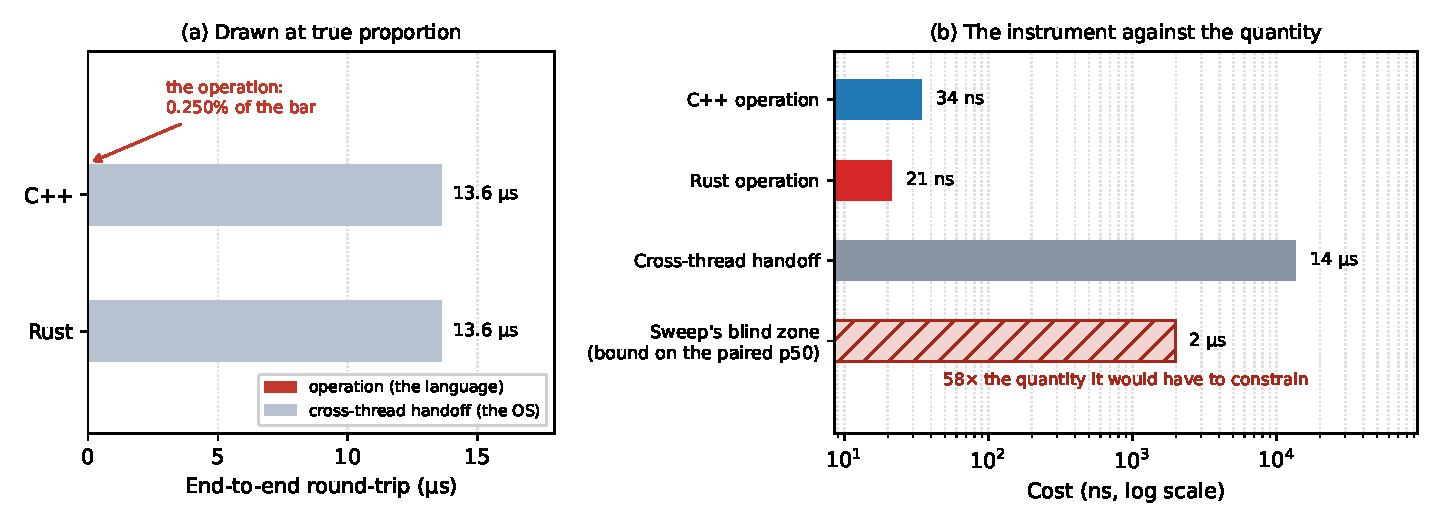
\includegraphics[width=0.78\linewidth]{figures/fig_budget.pdf}
\caption[Thao tác end-to-end được phân rã, so với sweep có thể giải quyết]{Chi phí end-to-end thao tác đi đâu, và vì sao sweep không bound hiệu ứng
ngôn ngữ. \textbf{(a)} Vòng quay theo tỷ lệ thật: thao tác ngôn ngữ thực hiện là
$\BudgetCoreShareMax\%$ thanh, phần còn lại handoff qua luồng. \textbf{(b)} Cùng đại lượng trên trục log so với hiệu ghép nhỏ nhất sweep có thể giải quyết,
hiển thị là vùng mù. Cả hai phép đo thao tác nằm trong nó bằng hệ số
$\BudgetBoundVsCore$, và (b) cũng là nơi khác biệt thời gian duy nhất chiến dịch giải quyết
nằm.\label{fig:budget}}
\end{figure}

Gán nhận cần cẩn thận, vì cách đọc tự nhiên là sai. Không gì ở đây
liên quan borrow checker, kiểm tra bound, hay ownership. Nguồn có thể nhất
đã ghi trong log điểm bắt buộc Bảng~\ref{tab:idioms}. Container mỗi shard là
hash map chuẩn của mỗi ngôn ngữ, và chúng là cấu trúc dữ liệu khác. \texttt{std::unordered\_map} của C++ phải node-based để giữ cam kết ổn định iterator và reference,
nên lookup đuổi pointer từ mảng bucket ra node cấp phát riêng. \texttt{HashMap} của Rust là bảng open-addressed giữ entry inline và
thường giải quyết lookup trong một cache line. Hàm hash được ghim FNV-1a cả hai
bên (Mục~\ref{sec:impldetails}) chính xác để hashing không thể là giải thích,
để lại bố cục container. Đó là khác biệt thật và có thể báo giữa hai
ngôn ngữ như thực tế dùng, vì developer chọn hash map chuẩn nhận
cái ngôn ngữ họ ship. Không phải bằng chứng về mô hình an toàn Rust và không
nên trích như vậy. Xác nhận cơ chế cần counter cache-miss
Mục~\ref{sec:threats} liệt kê là khoảng instrumentation rõ nhất.

Ba giới hạn giữ phát hiện đúng kích thước. Đó là microbenchmark một luồng, không tranh chấp,
nên nói thao tác tốn bao nhiêu chứ không hệ tải làm gì với nó. Đo trên cùng host sweep, nên số tuyệt đối mang cùng cảnh báo, dù tỷ số ít nhạy hơn mỗi thành phần. Và đó là một
thao tác trên một cấu trúc dữ liệu. Tổng quát hóa thành ``Rust nhanh $\BudgetCoreRatio\times$
hơn'' sẽ lặp chính lỗi luận văn này chỉ trích trong literature trường hợp trung bình.

\subsection{Độ trễ, throughput và bão hòa qua sweep}
Hình~\ref{fig:latency-load} vẽ p99 độ trễ so với tải đề nghị, và hình dạng là
hình Hình~\ref{fig:cliff} phác. Qua vùng tracking bốn variant leo
cùng nhau và nhẹ, từ khoảng $240\,\mu$s ở tải nhẹ tới single-digit millisecond
bởi $\SatKnee$~kops/s. Dải tin cậy ở đó đủ rộng để không curve tách
khỏi curve khác ở vùng đó. Sau đó, trong một bước duy nhất của thang tốc độ tiếp theo,
p99 mọi variant tăng hơn hai bậc magnitude cùng lúc, từ khoảng $6$~ms tới
vài giây. Đó là vách quá tải, và mức đột ngột đến là phát hiện. Một
bước tăng tải đề nghị tách dịch vụ đáp ứng deadline millisecond khỏi dịch vụ lỡ
ba bậc magnitude. Thiết kế với hàng đợi chặn có giới hạn không có suy giảm nhẹ nhàng
ở giữa.

Hai tính chất phía xa vách giới hạn ý nghĩa số, và chúng là lý do
Mục~\ref{sec:stats} không test percentile ở đó. Độ trễ qua knee là backlog
lịch tích chứ không phải thời gian phục vụ. Và vì giai đoạn đo bị cắt ở
chiều rộng cố định, percentile báo cáo bão hòa gần chiều rộng đó, làm mọi percentile
trên knee là bound dưới. Điều còn diễn giải được trong regime này là mỗi variant
vẫn hoàn tất bao nhiêu việc, và Mục~\ref{sec:overload} nói tiếp.

\begin{figure}[ht]
\centering
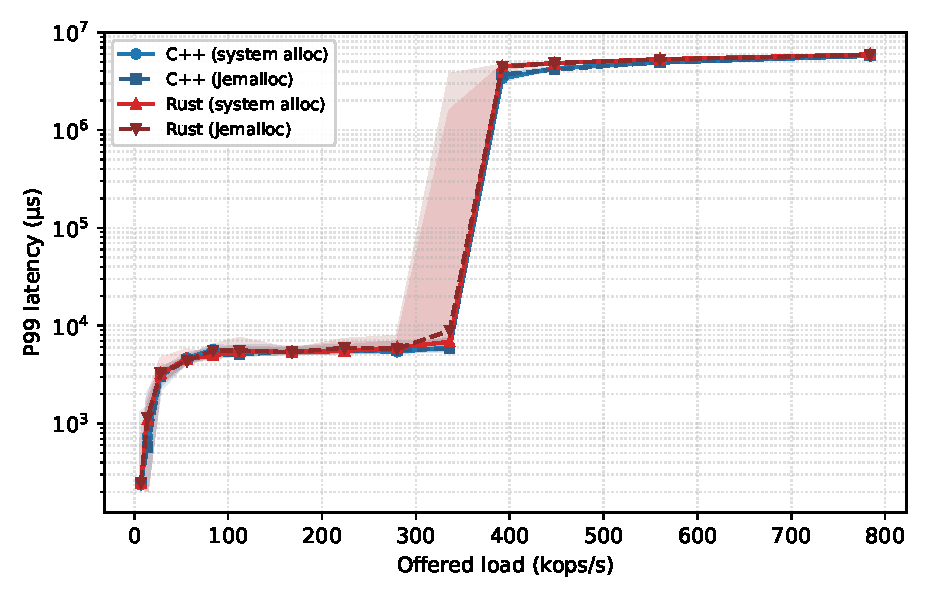
\includegraphics[width=0.66\linewidth]{figures/fig_latency_vs_load.pdf}
\caption[Độ trễ đuôi so với tải đề nghị]{Độ trễ đuôi (p99) so với tải đề nghị cho bốn variant build. Đường là median
qua \NRepeats{} lần lặp. Dải shaded là CI bootstrap $95\%$. Trục $y$ log.
\label{fig:latency-load}}
\end{figure}

Hình~\ref{fig:throughput-load} cho throughput đạt so với tải đề nghị, và là
plot thông tin hơn. Throughput là trung bình cả lần chạy, làm nó ít
nhạy hơn percentile với nhiễu rơi vào thao tác riêng lẻ.
Mọi variant bám đường lý tưởng đề nghị-bằng-đạt tới $\TrackingLoad$~kops/s và
bão hòa khoảng $\SatKnee$~kops/s. Hai điều theo ngay. Thứ nhất, throughput đạt
khớp tải đề nghị dưới knee trong $\ReprLoadShortfall\%$, nên điểm vận hành
Bảng~\ref{tab:latency} là tải \emph{bền vững} thật chứ không danh nghĩa.
Độ trễ báo ở đó không phải của hệ đã xếp hàng. Thứ hai, knee
nằm cùng chỗ cho cả bốn variant, điều cấu trúc một luồng mỗi shard
dự đoán. Nơi thiết kế không còn chịu là tính chất thiết kế.

Điều xảy ra \emph{sau} knee không được chia sẻ. Bốn curve tách ngay khi
tốc độ đề nghị không còn đáp ứng, và tách theo ngôn ngữ chứ không theo bộ cấp phát.
Mục~\ref{sec:overload} đo phân tách đó thay vì để mắt.

\begin{figure}[ht]
\centering
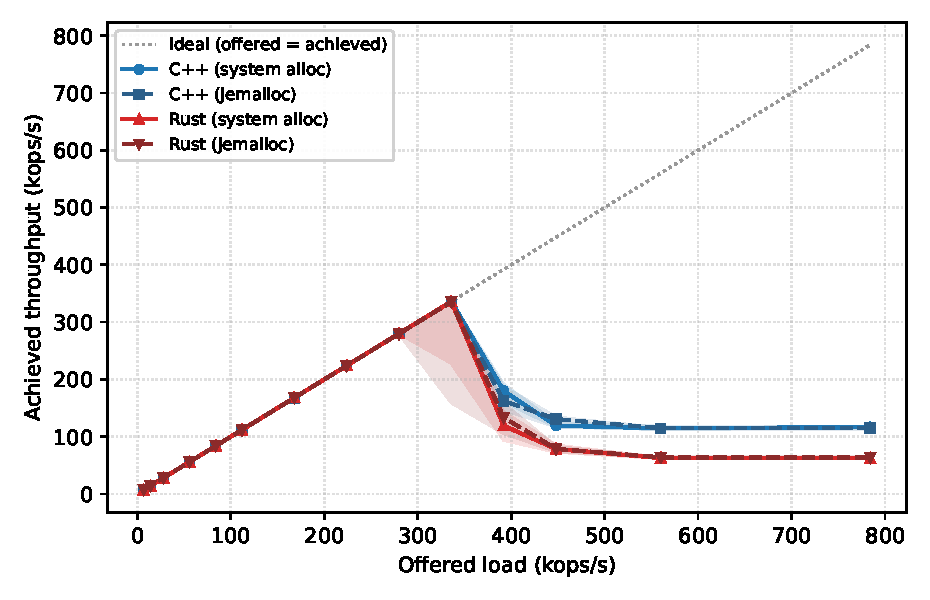
\includegraphics[width=0.66\linewidth]{figures/fig_throughput_vs_load.pdf}
\caption[Throughput đạt so với tải đề nghị]{Throughput đạt so với tải đề nghị. Đường chấm đánh dấu regime lý tưởng
đề nghị-bằng-đạt. Throughput được đếm chỉ trong giai đoạn đo, nên warm-up
không thiên cả mẫu số và tử số.\label{fig:throughput-load}}
\end{figure}

Hình~\ref{fig:tailpct} giữ tải cố định và sweep percentile. Bốn
variant trùng ở median và tỏ ra khi percentile tăng. Đó là hình dạng mong đợi
cho phân phối heavy-tailed, và là lý do methodology nhận biết percentile dùng xuyên suốt.
Tỏ ra không phải hiệu ứng ngôn ngữ, và panel phải cho thấy vì sao. Nó đặt spread
giữa bốn variant ở mỗi percentile so với khoảng rộng nhất một variant
mang ở đó. Ở median spread là lớn hơn của hai, regime
trong đó thứ tự có nghĩa. Từ p90 trở lên khoảng vượt spread nhiều lần. Sự tỏ ra do đó đánh dấu nơi phép đo mất độ phân giải, không nơi
ngôn ngữ khác.

\begin{figure}[ht]
\centering
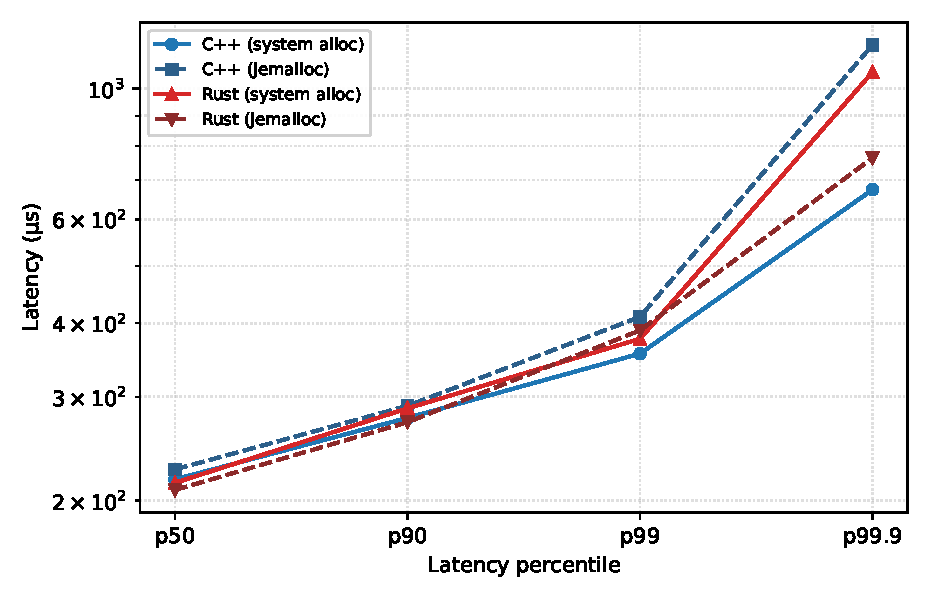
\includegraphics[width=0.78\linewidth]{figures/fig_tail_percentiles.pdf}
\caption[Độ trễ qua dải percentile, và giới hạn host]{Độ trễ mỗi thao tác qua dải percentile ở $\ReprLoad$~kops/s. \textbf{(a)} Bốn
variant là median qua \NRepeats{} lần lặp, mỗi cái với dải bootstrap $95\%$. Dải
là điểm: vẽ đường trần các curve chồng lên và đọc như tuyên bố
tương đương, không phải điều phép đo không thể tách đã chứng minh. \textbf{(b)}
Vì sao không thể tách trên median. Spread giữa bốn variant được đặt
so với khoảng tin cậy rộng nhất trên bất kỳ một variant, với tỷ số chú thích trên mỗi
cặp thanh. Khi tỷ số vượt một, uncertainty về một variant lớn hơn
khoảng giữa cả bốn và không thứ tự nào đọc được.\label{fig:tailpct}}
\end{figure}

\subsection{Hành vi qua bão hòa (RQ1)}\label{sec:overload}
RQ1 hỏi hai ngôn ngữ so với nhau thế nào khi tải tăng \emph{và quá tải}, và mọi thứ
báo trước đó ở dưới knee. Mục này là nửa kia. Điểm vận hành là
$\OverloadLoad$~kops/s đề nghị, định nghĩa là tải sweep sâu nhất mà mọi variant đã
ngừng đáp ứng tốc độ đề nghị, và metric là hai cái còn diễn giải được ở đó
(Mục~\ref{sec:stats}). Bảng~\ref{tab:overload} cho mỗi variant vẫn duy trì gì và
Bảng~\ref{tab:overloadtest} test so sánh.

Ngôn ngữ không tương đương trong regime này, và margin không nhỏ.
\OverloadSustainedFaster{} duy trì $\OverloadThrCpp$~kops/s trong khi \OverloadSustainedSlower{}
duy trì $\OverloadThrRust$, hệ số $\OverloadThrRatio$. Hiệu ghép ít nhất
$\OverloadThrBound$~kops/s dưới cả hai bộ cấp phát, giữ trong \OverloadThrAgree{} lần lặp, và
$p$ Holm của nó ở sàn hiệu chỉnh của cả họ \NTests{} test. Đây là
hiệu ứng ngôn ngữ lớn nhất và tái lập nhất trong nghiên cứu, và là cái duy nhất
nói trực tiếp câu hỏi RQ1 được viết để hỏi.

Cột CPU là điều làm kết quả diễn giải được chứ không chỉ lớn, vì nó loại
cách đọc tự nhiên nếu không. Variant hoàn tất ít việc hơn có thể đơn giản
làm ít hơn: bị throttle, chặn, rảnh. Không phải vậy.
\OverloadSustainedSlower{} dùng \emph{nhiều} CPU tổng hơn \OverloadSustainedFaster{} ở đây,
tái lập và dưới cả hai bộ cấp phát, đã đảo dấu nó mang ở tải đại diện
Bảng~\ref{tab:significance}. Chia qua việc thực sự hoàn tất, chi phí CPU mỗi thao tác duy trì là $\OverloadCpuPerOpRatio$ lần bên kia. Không
variant gần capacity máy, vì cả hai ở khoảng sáu trong mười bốn lõi ghim.
Gap do đó không phải giới hạn capacity và không phải rảnh. Đó là effort tiêu không hoàn tất
thao tác, dấu hiệu đường đồng bộ quay, hoặc park và
wake lặp, nơi bên kia chặn một lần và ngủ.

Hình~\ref{fig:overload} đặt cả hai nửa cách đọc cạnh nhau, và nhóm mang
thứ ba. Phân tách gần như hoàn toàn trong nhóm bộ cấp phát, nghĩa hiệu ứng
theo biến nghiên cứu thao tác chứ không biến đối chứng.

\begin{figure}[ht]
\centering
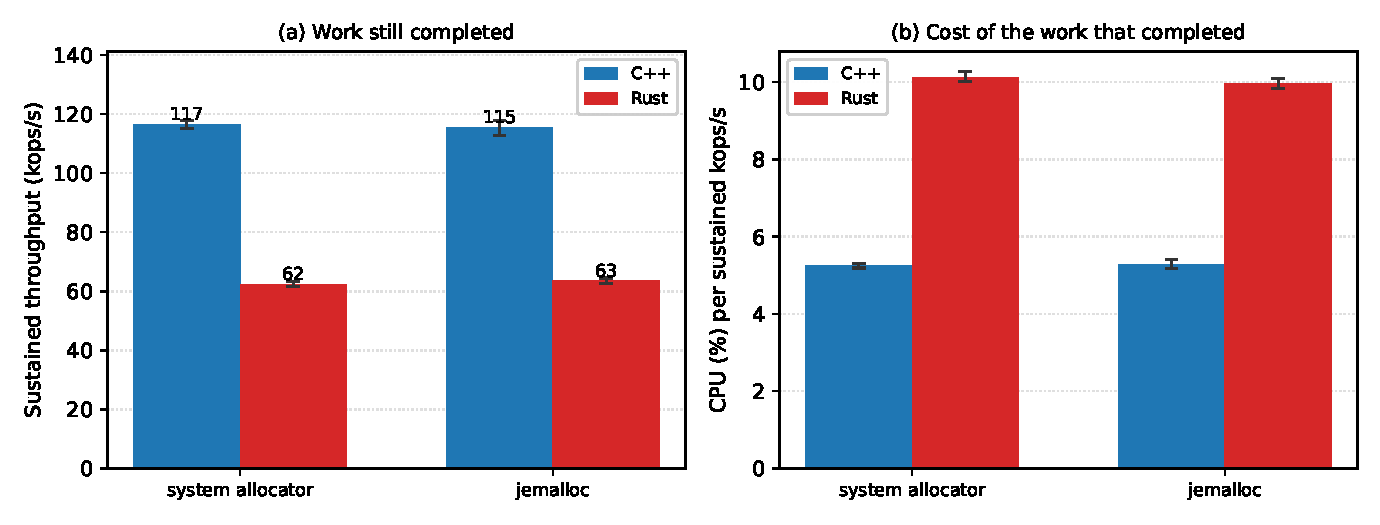
\includegraphics[width=0.78\linewidth]{figures/fig_overload.pdf}
\caption[Phân kỳ qua bão hòa]{Hành vi ở $\OverloadLoad$~kops/s đề nghị, xa quá knee $\SatKnee$~kops/s. Thanh
là median qua \NRepeats{} lần lặp với khoảng bootstrap $95\%$, nhóm sao cho hai
thanh trong nhóm chỉ khác ngôn ngữ. \textbf{(a)} Mỗi variant vẫn hoàn tất:
\OverloadSustainedFaster{} duy trì hệ số $\OverloadThrRatio$ hơn
\OverloadSustainedSlower. \textbf{(b)} Tổng CPU chia cho việc thực sự hoàn tất, điều loại
cách đọc variant giao ít hơn đơn giản làm ít hơn. Nó tiêu
$\OverloadCpuPerOpRatio$ lần CPU mỗi thao tác duy trì, và số CPU
được cộng qua luồng.\label{fig:overload}}
\end{figure}

Effort đi đâu được thu hẹp bằng phép đo chứ không để mở. Qua
bão hòa producer tiêu gần hết thời gian ở hai chỗ ghi trong
Bảng~\ref{tab:idioms}: hàng đợi chặn có giới hạn và tay cầm hoàn tất.
Mục~\ref{sec:contention} cô lập các nguyên thủy đó, và chúng không tái tạo
thứ tự full-service ở mức ý nghĩa. Điều đó loại chúng \emph{riêng lẻ} làm toàn bộ giải thích
cho gap $\OverloadThrRatio\times$. Như Mục~\ref{sec:budget}, không gì trong borrow checker,
kiểm tra bound, hay ownership bị liên quan, và phát hiện không nên trích như
là.

Ba điều lại giới hạn phát hiện cho phép gì. Đó là một thiết kế, dịch vụ shared-nothing với một
yêu cần outstanding mỗi producer và giới hạn hàng đợi $1\,024$, và độ sâu sụp đổ
phụ thuộc cả ba. Đo với harness có producer chặn mỗi yêu cầu, nên nó
mô tả client hình dạng này trải nghiệm chứ không client pipeline.
Và số tuyệt đối thuộc host này. Điều đi theo là thứ tự và nguyên nhân. Dưới
bão hòa lựa chọn ngôn ngữ không quan trọng. Trên nó nguyên thủy đồng bộ thư viện chuẩn
quan trọng, và crossover đủ sắc để so sánh dừng ở tải danh nghĩa
sẽ kết luận ngược.

Crossover cũng liên quan công trình trước gần nhất, báo suy giảm tương đương qua
ngưỡng tốc độ yêu cầu và gán cho runtime async~\cite{arvidsson2025async}. Mục~\ref{sec:rqdiscussion} nói ý nghĩa khi
cùng hình dạng xuất hiện ở đây không có runtime như vậy ở cả hai bên.

\begin{table}[H]
\centering
\small
\caption[Mỗi variant vẫn duy trì gì qua bão hòa]{Mỗi variant vẫn duy trì ở
$\OverloadLoad$~kops/s đề nghị, xa quá knee $\SatKnee$~kops/s: median qua
\NRepeats{} lần lặp trên khoảng tin cậy bootstrap $95\%$. Dưới bão hòa throughput đạt
bị ghim tốc độ đề nghị theo cấu trúc và không thể nói gì về
ngôn ngữ. Ở đây đó là thứ duy nhất có thể. Sử dụng CPU vượt $100\%$ vì được
cộng qua luồng, nên $600\%$ là sáu lõi bận trong mười bốn
ghim.\label{tab:overload}}
\begin{tabular}{@{}l r r@{}}
\hline\hline
Variant & sustained throughput (kops/s) & CPU (\%) \\
\hline
C++ (system alloc) & \mci{146.7}{146.3}{147.2} & \mci{662.8}{662.5}{663.6} \\
C++ (jemalloc) & \mci{146.4}{146.1}{146.9} & \mci{664.3}{663.3}{664.9} \\
Rust (system alloc) & \mci{84.5}{84.2}{84.7} & \mci{681.8}{680.4}{682.5} \\
Rust (jemalloc) & \mci{84.3}{83.9}{84.6} & \mci{680.3}{679.8}{681.5}
\\
\hline
\end{tabular}
\end{table}

\begin{table}[H]
\centering
\small
\caption[Test ghép chính xác qua bão hòa]{Test ghép hoán vị chính xác C++ so với Rust ở
$\OverloadLoad$~kops/s, bộ cấp phát giữ cố định, hiệu chỉnh Holm trên cùng họ
\NTests{} test như Bảng~\ref{tab:significance} chứ không là họ riêng. ``Repeats''
đếm bao nhiêu trong \NRepeats{} hiệu ghép đồng ý dấu median, điều statistic tính từ mean không thể hiện. Không percentile độ trễ được test ở đây, vì
lý do cố định trước Mục~\ref{sec:stats}.\label{tab:overloadtest}}
% The generated metric names are long enough that six l/r columns overrun the text
% block; the first column wraps instead, and the inter-column padding is tightened.
\setlength{\tabcolsep}{4pt}
\begin{tabular}{@{}p{0.24\linewidth} l r c r r@{}}
\hline\hline
Metric & Allocator & Effect (Rust $-$ C++) & Repeats & $p$ & Holm \\
\hline
Sustained throughput (kops/s) & system & \mci{-62.2}{-62.9}{-61.6} & 20/20 & 0.0000019 & 0.000027 \\
Sustained throughput (kops/s) & jemalloc & \mci{-62.2}{-62.7}{-61.6} & 20/20 & 0.0000019 & 0.000027 \\
CPU utilisation (\%) & system & \mci{+19.5}{+17.3}{+19.9} & 20/20 & 0.0000019 & 0.000027 \\
CPU utilisation (\%) & jemalloc & \mci{+16.8}{+15.6}{+17.5} & 20/20 & 0.0000019 & 0.000027
\\
\hline
\end{tabular}
\end{table}
